\textit{Response.}

\begin{enumerate}[a)]
	\item We will utilize the observation model
	
	\begin{equation}
		v_{k+1} = g\,u_{k+1} + \sigma^{o}\,\zeta_{k+1}
	\end{equation}
	
	where $k$ is the time-step index.
	
	Source code is available from the GitHub repository
	
	\begin{center}
		\url{https://github.com/jasonltorchinsky/MATH833_HW/releases/tag/hw4}
	\end{center}

	and is given in Appendix~\ref{app:code_3a}. In short, the code takes a input parameters \texttt{-a}, \texttt{-f}, \texttt{-s}, \texttt{-g}, and \texttt{-z}, which correspond to $a$, $f$, $\sigma$, $g$, and $\sigma^{o}$, respectively. The code then simulates 250 individual realizations of the linear stochastic differential equation (SDE) (and observations of those realizations) using the Euler--Maruyama method with time-step size $\Delta t = 0.01$, and generates the plots included below
	
	\begin{figure}[H]
		\centering
		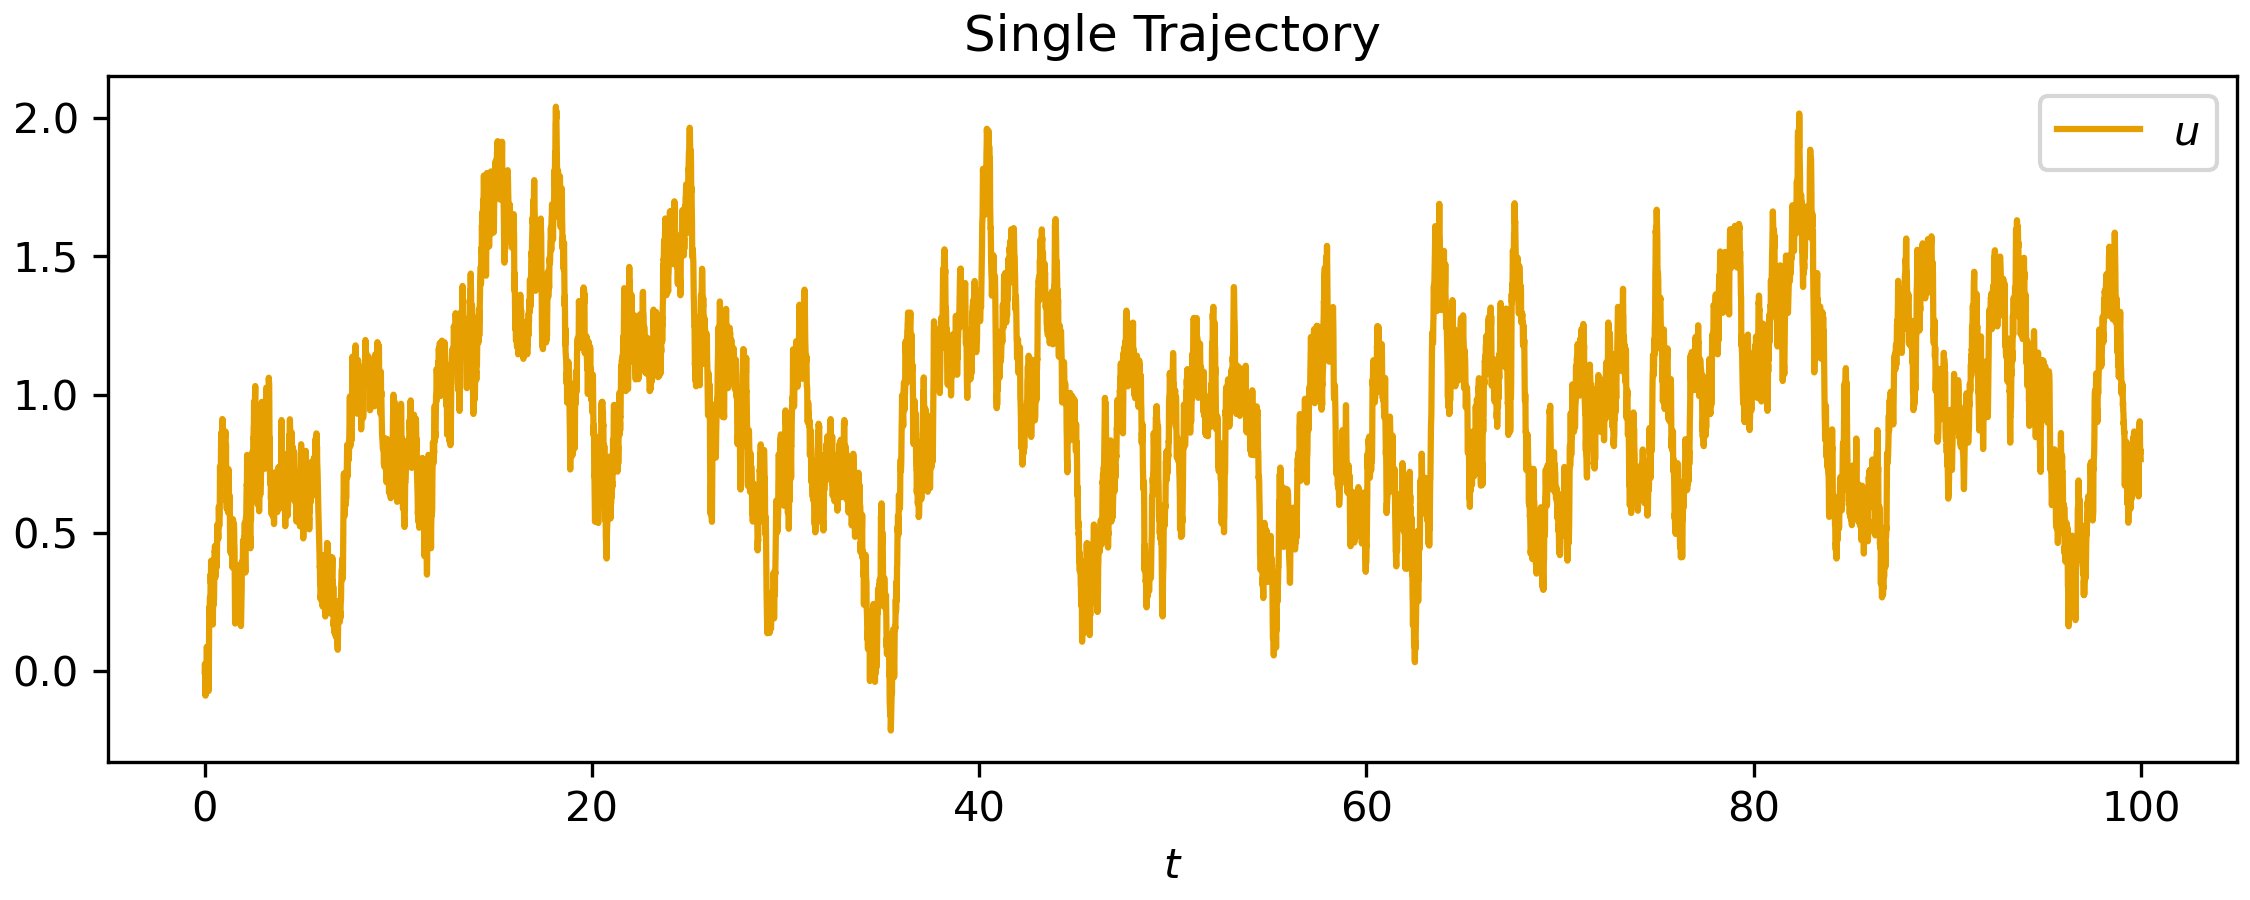
\includegraphics[width=0.75\textwidth]{../../src/3a_traj.png}
		\caption{A single realization of the SDE (top) and the difference between the observed and `true' values of $u$ (bottom) with parameters $a = f = 1$ and $\sigma = 0.5$ with initial condition $u = 0$ and time-step size $\Delta t = 0.01$. }
		\label{fig:3a_traj}
	\end{figure}
	
	\begin{figure}[H]
		\centering
		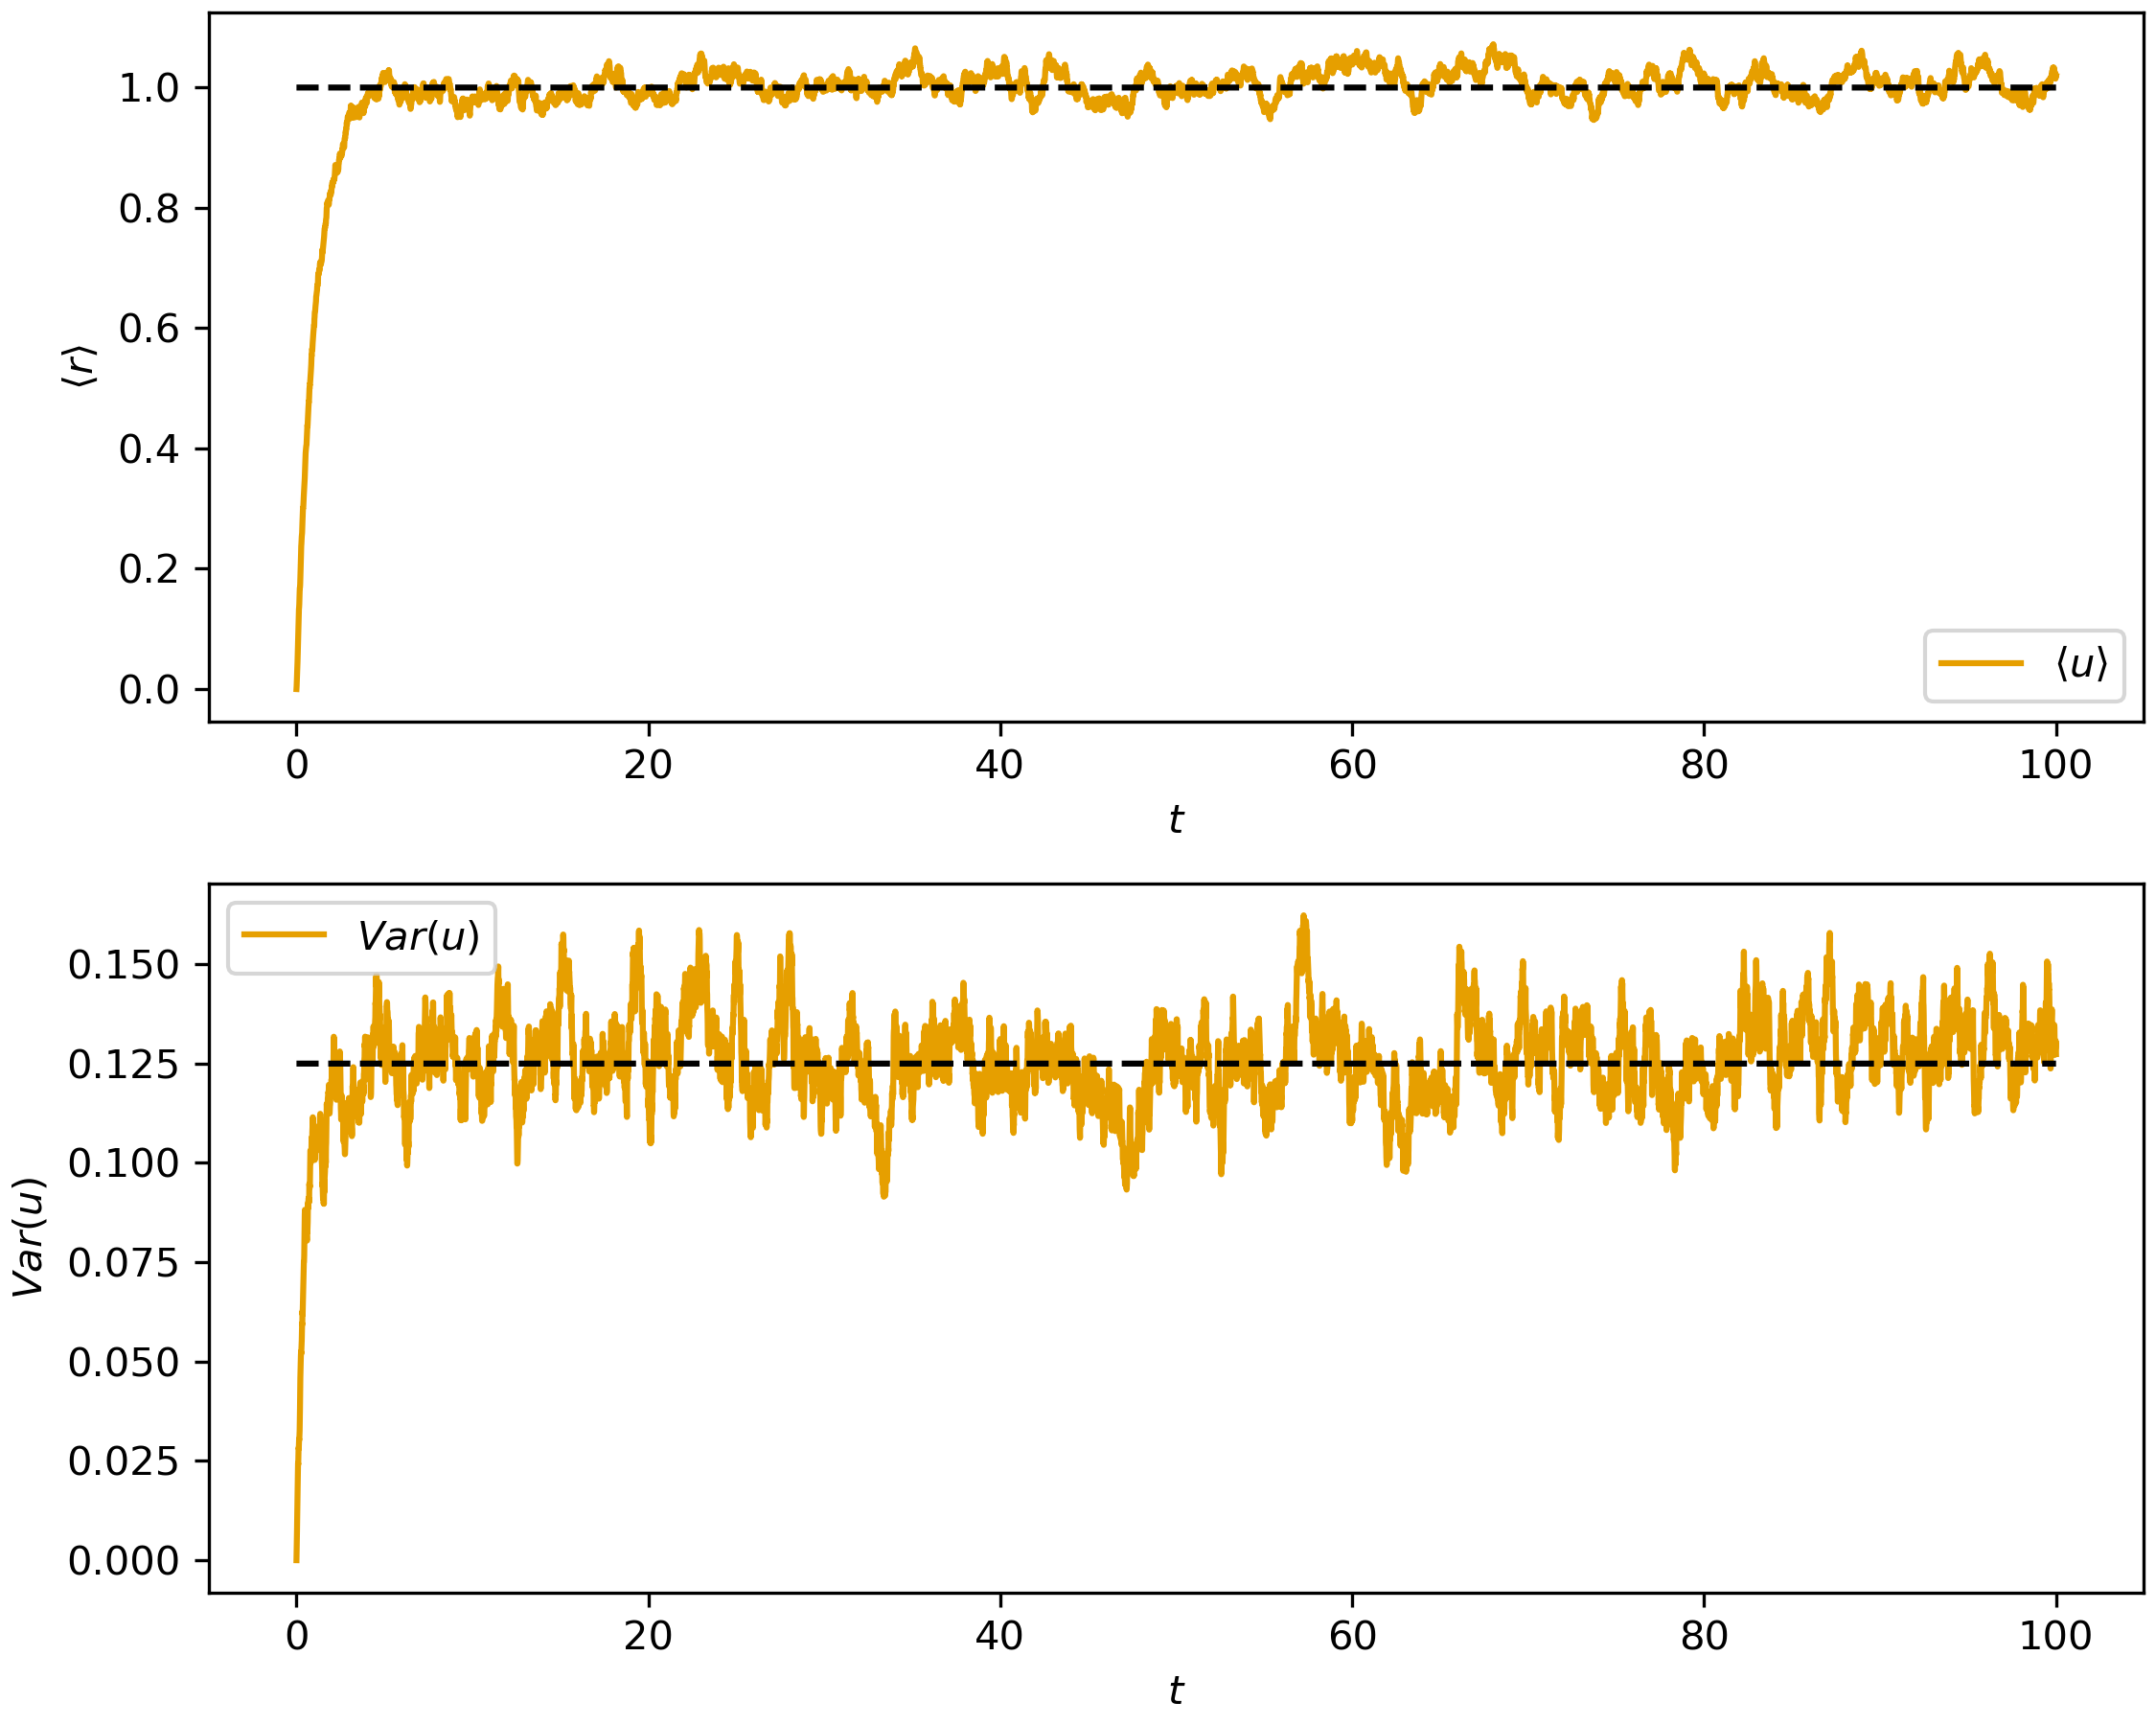
\includegraphics[width=0.75\textwidth]{../../src/3a_ens_stats.png}
		\caption{The evolution of ensemble mean (top) and variance (bottom) of the SDE with parameters $a = f = 1$ and $\sigma = 0.5$ across 250 trials, with initial condition $u = 0$ and time-step size $\Delta t = 0.01$ for all trials. }
		\label{fig:3a_ens_stats}
	\end{figure}
	
	\item For this problem, we will utilize three distinct models: 1) the truth model
	
	\begin{equation}
		u_{k+1} = u_{k} + \gpr{-a\,u_{k} + f}\,\Delta t + \sigma\,\sqrt{\Delta t}\,\xi_{k+1}
	\end{equation}
	
	where $\xi_{k+1}$ is a sample from a zero-mean unit-variance normal distribution, 2) the `imperfect' model (an augmented version of the truth model)
	
	\begin{equation}
		\va{u}_{k+1 \vert k} = \va{u}_{k \vert k} + \vb{A}\,\va{u}_{k \vert k}\,\Delta t + \vb{\Sigma}\,\sqrt{\Delta t}\,\va{\xi}_{k+1}
	\end{equation}
	
	where
	
	\begin{equation}
		\va{u} = \mqty[u \\ f],\qquad \vb{A} = \mqty[-a & 1 \\ 0 & 0],\qquad \vb{\Sigma} = \mqty[\sigma & 0 \\ 0 & 0],
	\end{equation}
	
	and $\va{\xi}_{k+1}$ is a $2 \times 1$ vector of an independent realization of zero-mean unit-variance Guassian noise, and 3) the observation model
	
	\begin{equation}
		\va{v}_{k+1} = \vb{G}\,\va{u}_{k+1} + \vb{\Sigma}^{o}\,\va{\zeta}_{k+1}
	\end{equation}
	
	where 
	
	\begin{equation}
		\vb{G} = \mqty[g & 0],\qquad \vb{\Sigma}^{o} = \mqty[\sigma^{o}],
	\end{equation}
	
	and $\va{\zeta}_{k+1}$ is a $1 \times 1$ vector of zero-mean unit-variance Guassian noise.
	
	The evolution of the Kalman filter is then given by
	
	\begin{subequations}
		\begin{equation}
			\overline{\va{u}}_{k+1 \vert k} = \gpr{\vb*{\mathcal{I}} + \Delta t\,\vb{A}}\,\overline{\va{u}}_{k \vert k},\qquad \vb{\Sigma}_{k+1 \vert k} = \gpr{\vb*{\mathcal{I}} + \Delta t\,\vb{A}}\,\vb{\Sigma}_{k \vert k}\,\gpr{\vb*{\mathcal{I}} + \Delta t\,\vb{A}}^{-1} + \vb{\Sigma},
		\end{equation}
		\begin{equation}
			\va{u}_{k+1} = \gpr{\vb*{\mathcal{I}} + \Delta t\,\vb{A}}\,\va{u}_{k} + \vb{\Sigma}\,\sqrt{\Delta t}\,\va{\xi}_{k+1},\qquad \va{v}_{k+1} = \vb{G}\,\va{u}_{k+1} + \vb{\Sigma}^{o}\,\va{\zeta}_{k+1},
		\end{equation}
		\begin{equation}
			\overline{\va{u}}_{k+1 \vert k+1} = \overline{\va{u}}_{k+1 \vert k} + \vb{K}_{k+1}\,\gpr{\va{v}_{k+1} - \vb{G}\,\overline{\va{u}}_{k+1 \vert k}},\qquad \vb{\Sigma}_{k+1 \vert k+1} = \gpr{\vb*{\mathcal{I}} - \vb{K}_{k+1}\,\vb{G}}\,\vb{\Sigma}_{k+1 \vert k},
		\end{equation}
		\begin{equation}
			\vb{K}_{k+1} = \vb{\Sigma}_{k+1 \vert k}\,\vb{G}^T\,\gpr{\vb{G}\,\vb{\Sigma}_{k+1\ \vert\ k}\,\vb{G}^T + \vb{\Sigma}^{o}}^{-1},
		\end{equation}
	\end{subequations}	
	
	where $\vb*{\mathcal{I}}$ is the appropriately-sized identity matrix, $\overline{\va{u}}_{k+1 \vert k}$ and $\vb{\Sigma}_{k+1 \vert k}$ are the prior filter mean and covariance, $\overline{\va{u}}_{k+1 \vert k+1}$ and $\vb{\Sigma}_{k+1 \vert k+1}$ are the posterior filter mean and covariance, and $\vb{K}_{k+1}$ is the Kalman gain matrix. Below we include plots of the posterior mean and covariances of the filter
	
	\begin{figure}[H]
		\centering
		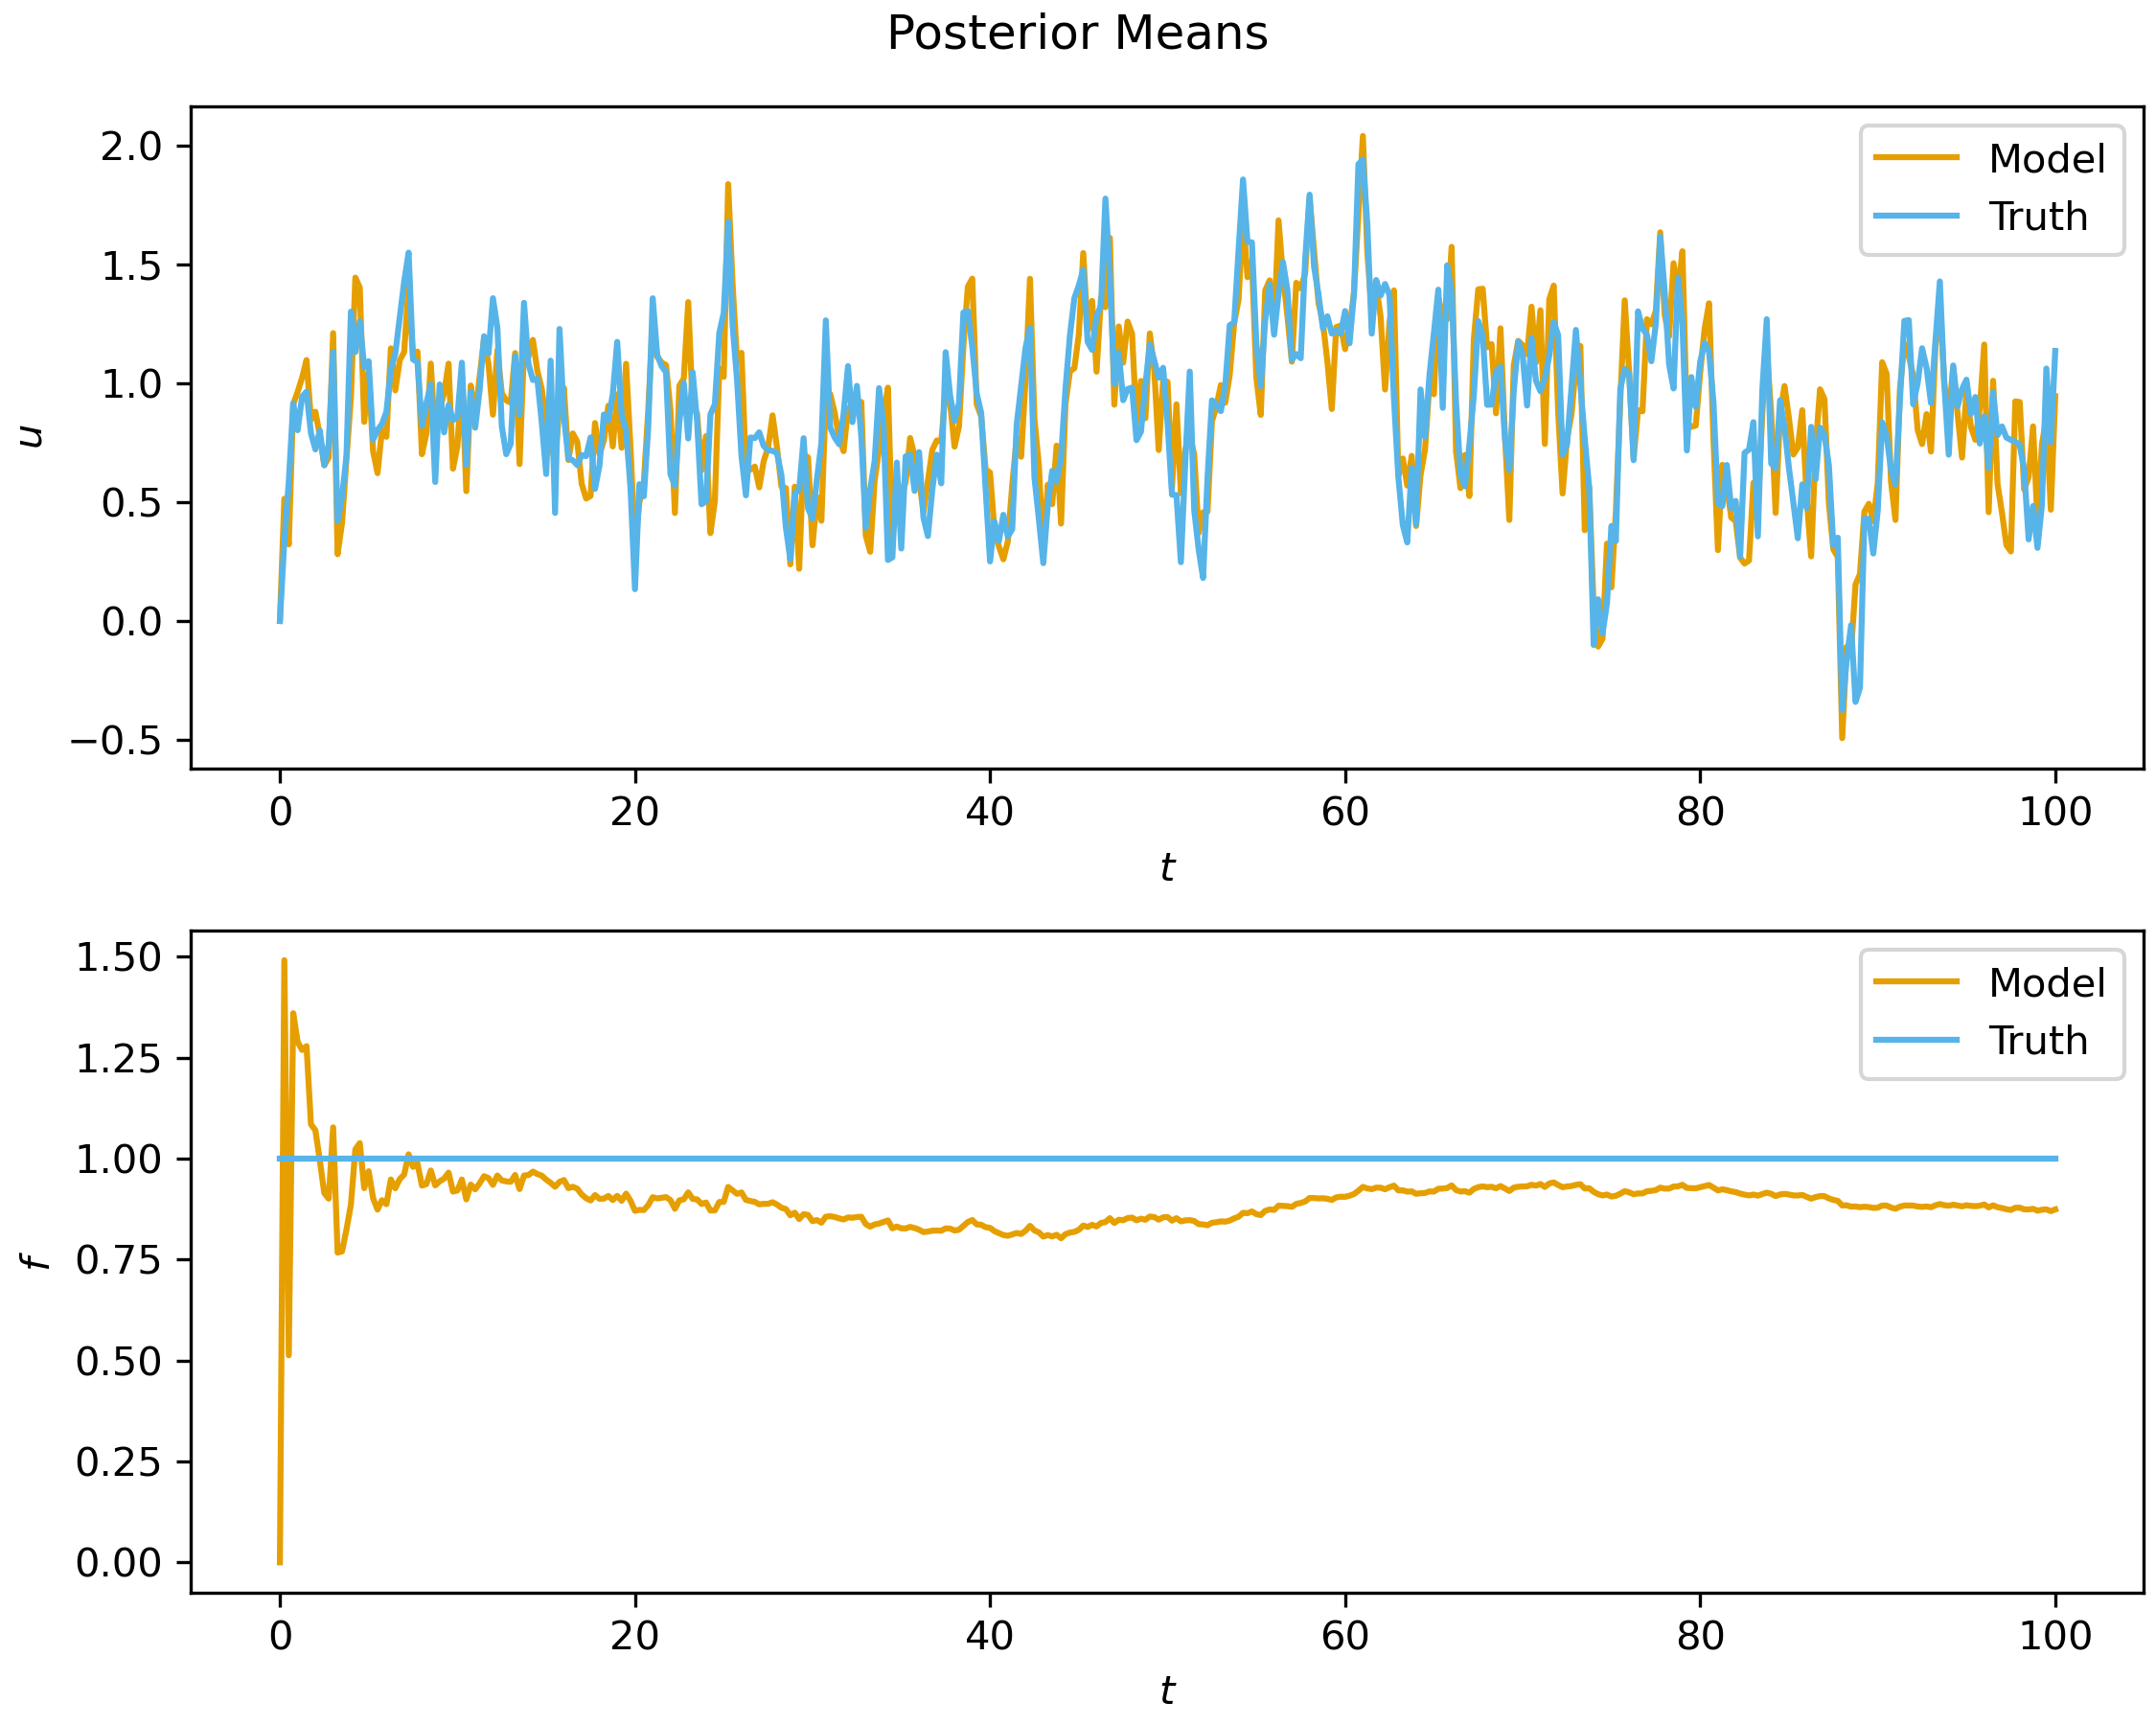
\includegraphics[width=0.75\textwidth]{../../src/3b_traj.png}
		\caption{The posterior means of the Kalman filter, with $u$ initialized as zero for both the truth and imperfect models, and $f$ initialized as zero for the imperfect model. The initial posterior covariance matrix of the filter was $\vb{\Sigma}_{0 \vert 0} = \mqty[1 & 1 \\ 1 & 50]$. The observation operator was $g = 1$ and observation noise strength was $\sigma^{o} = 0.25$.}
		\label{fig:3b_traj}
	\end{figure}
	
	\begin{figure}[H]
		\centering
		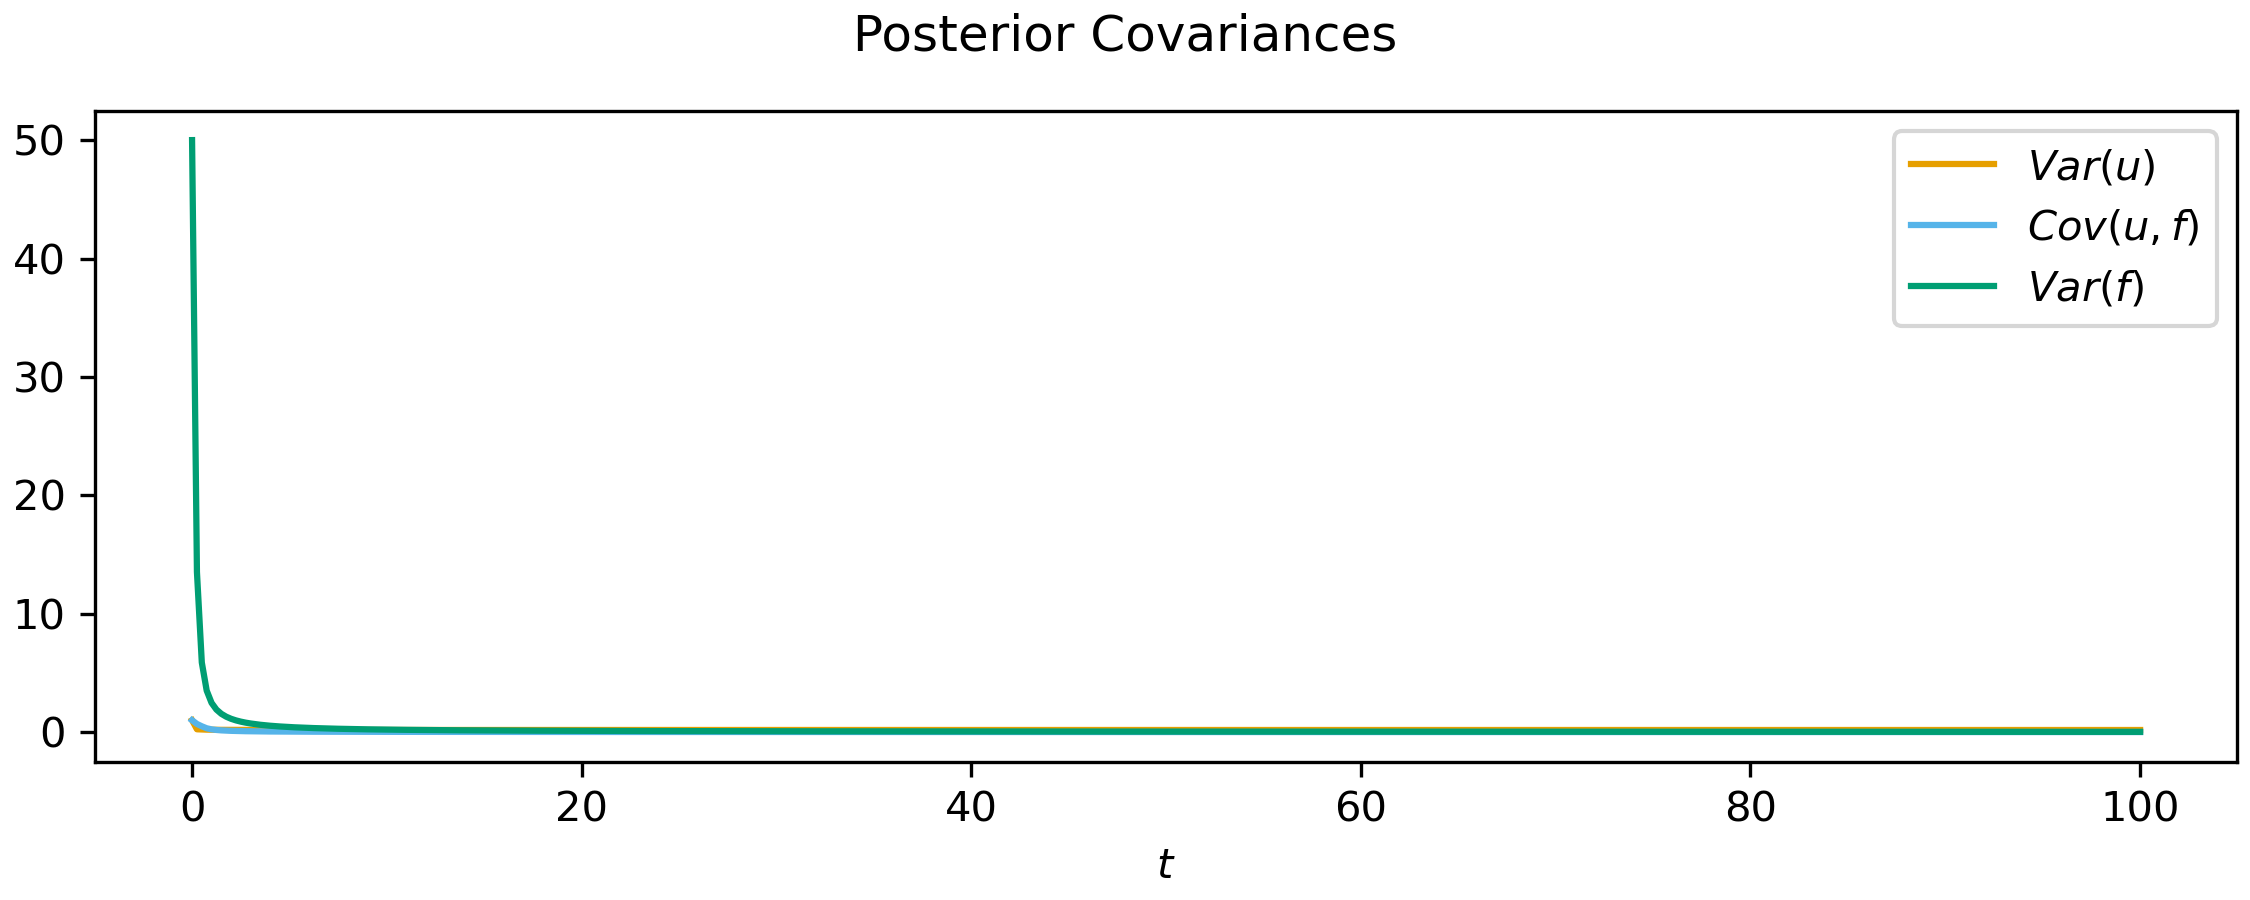
\includegraphics[width=0.75\textwidth]{../../src/3b_cov.png}
		\caption{The posterior covariances of the Kalman filter, with $u$ initialized as zero for both the truth and imperfect models, and $f$ initialized as zero for the imperfect model. The initial posterior covariance matrix of the filter was $\vb{\Sigma}_{0 \vert 0} = \mqty[1 & 1 \\ 1 & 50]$. The observation operator was $g = 1$ and observation noise strength was $\sigma^{o} = 0.25$.}
		\label{fig:3b_cov}
	\end{figure}
	
	Source code is available from the GitHub repository
	
	\begin{center}
		\url{https://github.com/jasonltorchinsky/MATH833_HW/releases/tag/hw4}
	\end{center}

	and is given in Appendix~\ref{app:code_3b}. In short, the code takes a input parameters \texttt{-a}, \texttt{-f}, \texttt{-s}, \texttt{-g}, and \texttt{-z}, which correspond to $a$, $f$, $\sigma$, $g$, and $\sigma^{o}$, respectively. The code then simulates one realization of the truth model, observations of the truth model, and a Kalman filter using the imperfect model using the Euler--Maruyama method with time-step size $\Delta t = 0.25$, and generates the plots included above.
	
	\item Below we include plots generate using the code from part b), except with $\Delta t = 0.01$.
	
	\begin{figure}[H]
		\centering
		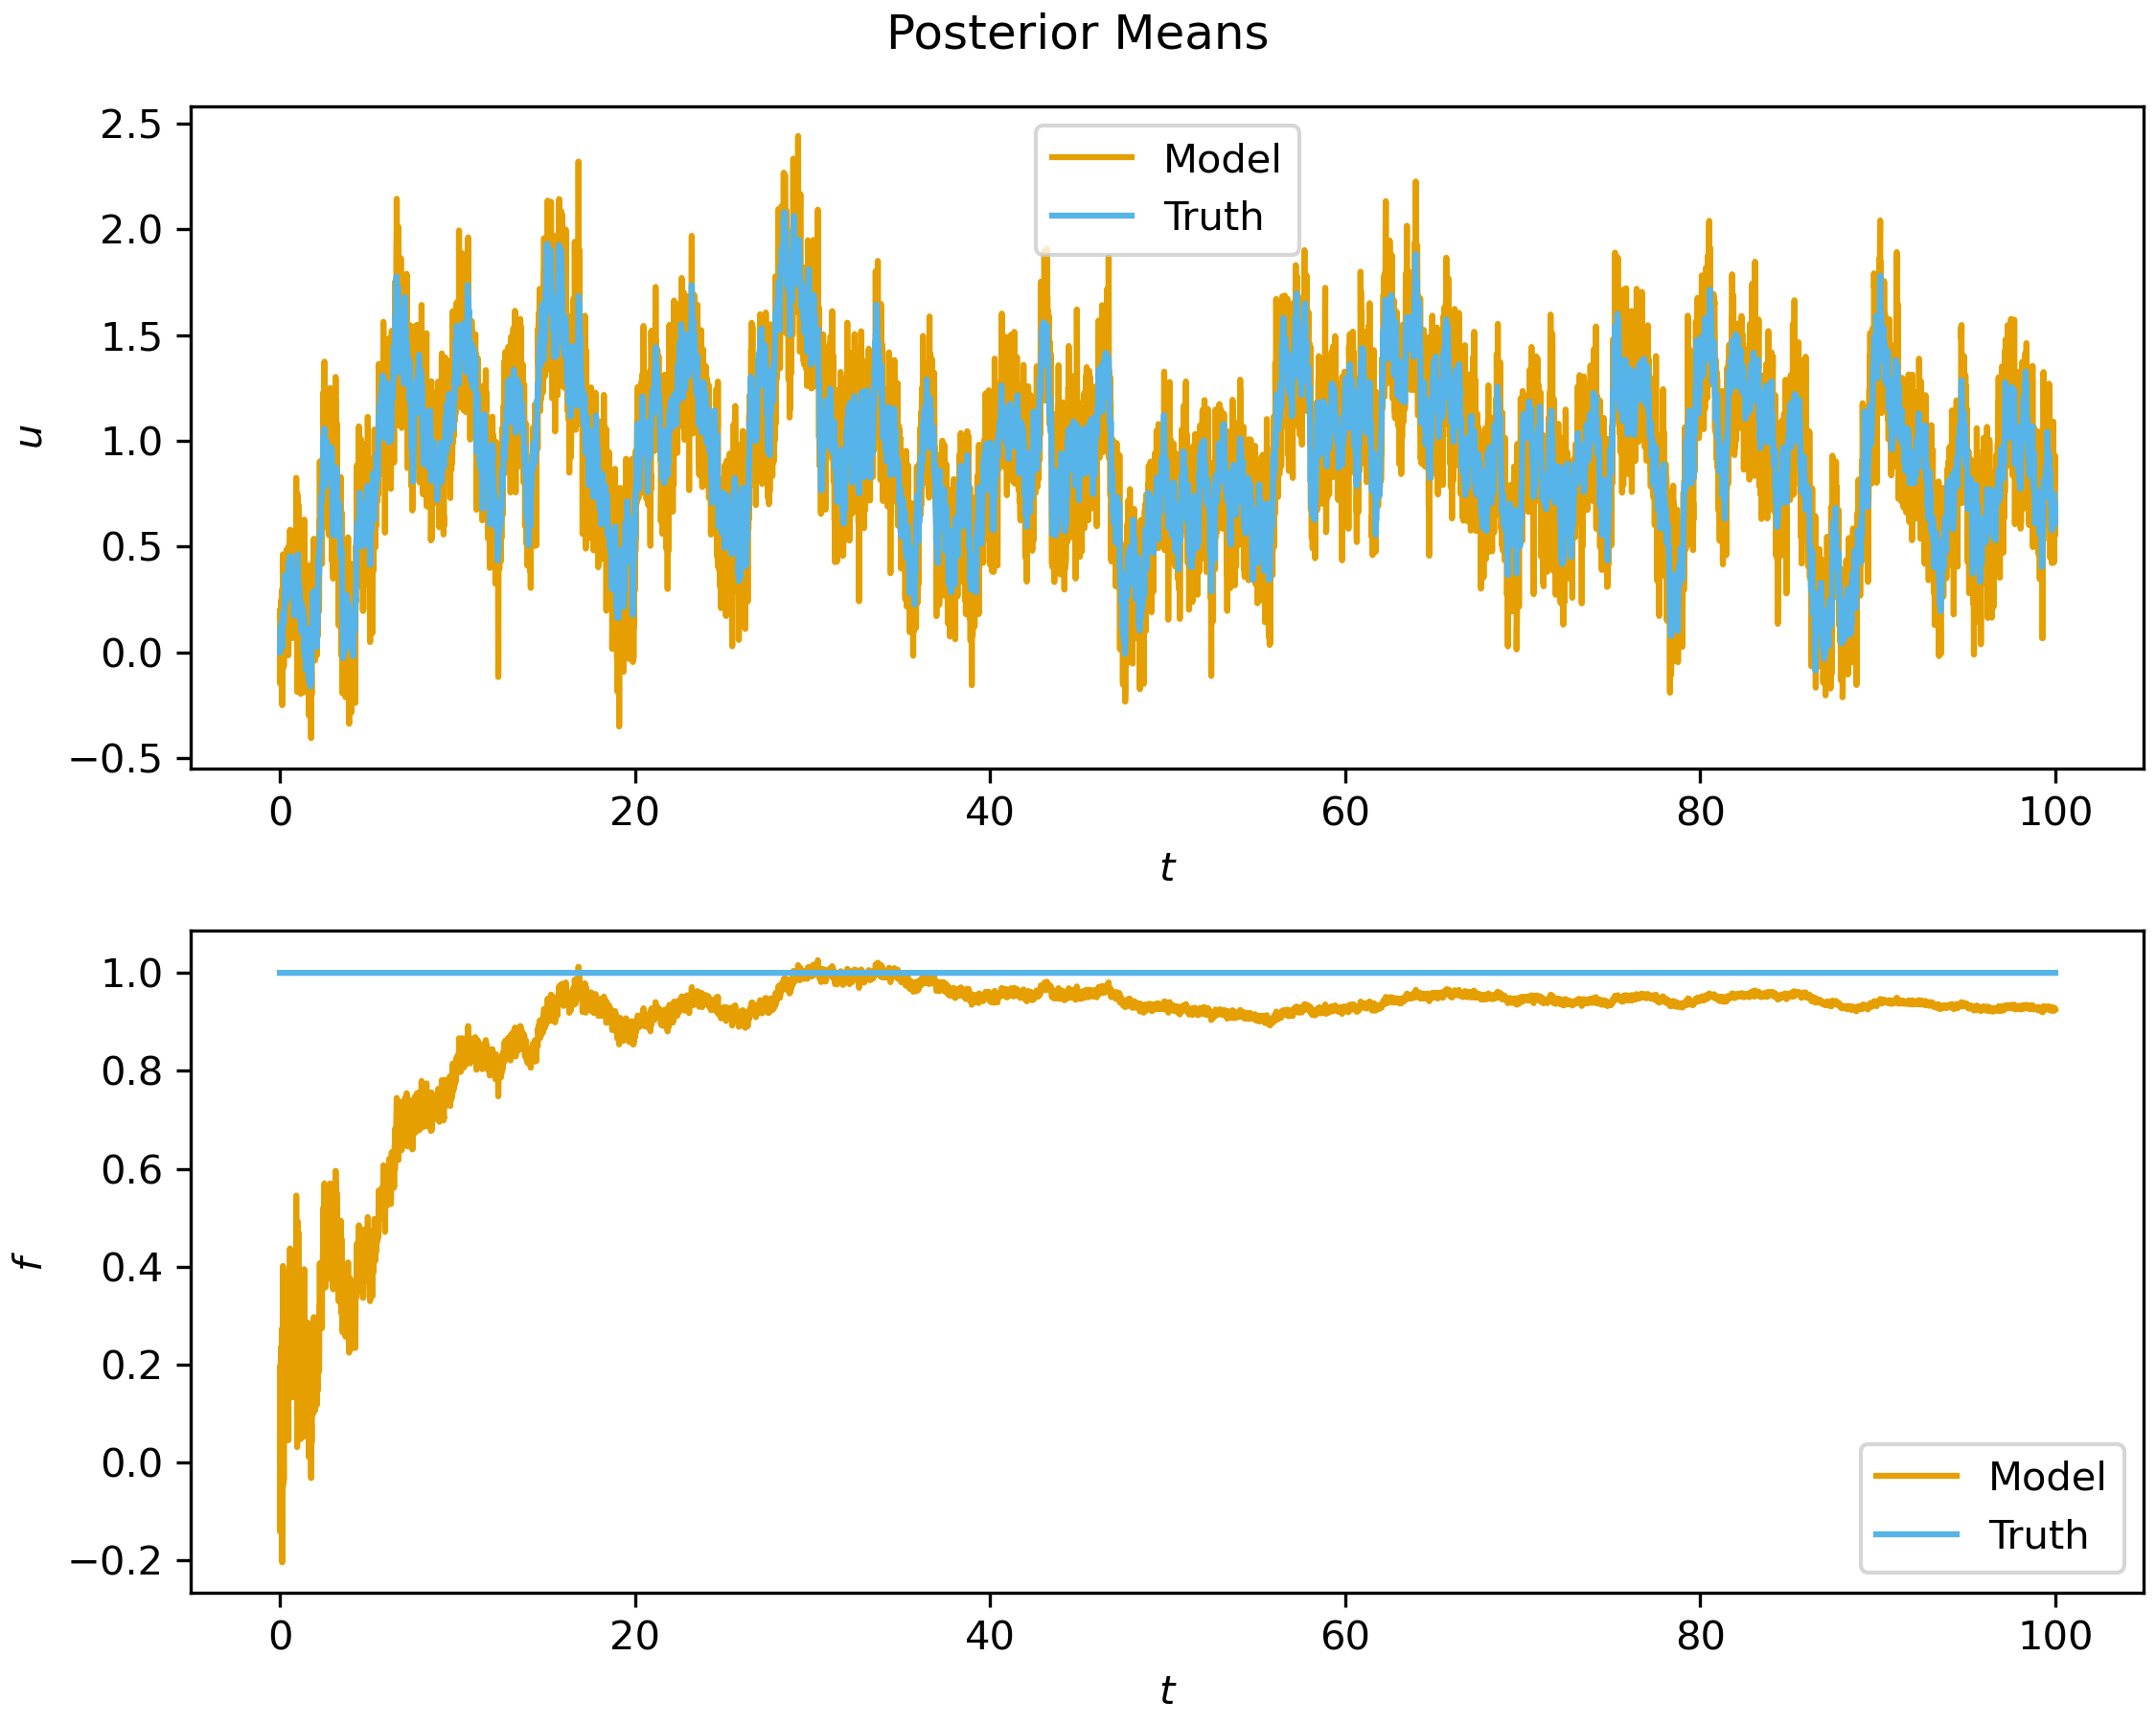
\includegraphics[width=0.75\textwidth]{../../src/3c_traj.png}
		\caption{The posterior means of the Kalman filter, with $u$ initialized as zero for both the truth and imperfect models, and $f$ initialized as zero for the imperfect model. The initial posterior covariance matrix of the filter was $\vb{\Sigma}_{0 \vert 0} = \mqty[1 & 1 \\ 1 & 50]$. The observation operator was $g = 1$ and observation noise strength was $\sigma^{o} = 0.25$.}
		\label{fig:3c_traj}
	\end{figure}
	
	\begin{figure}[H]
		\centering
		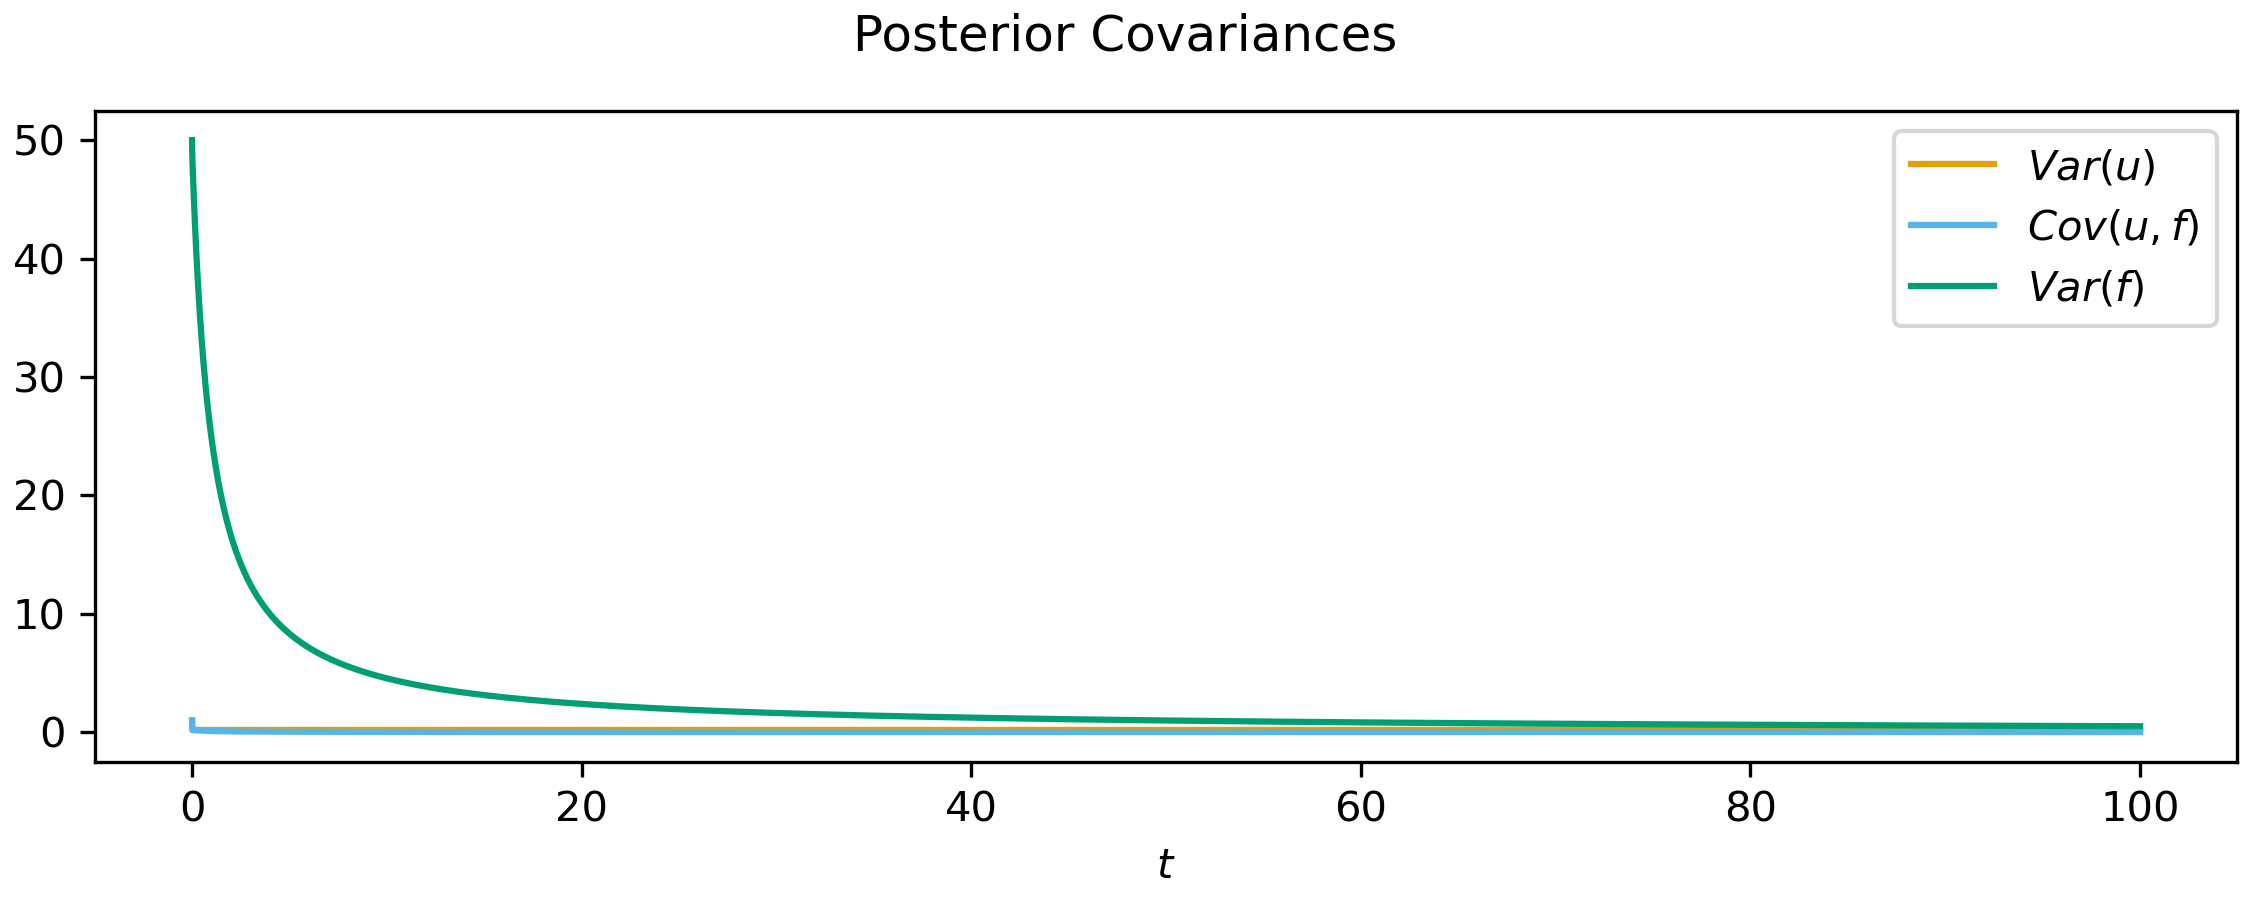
\includegraphics[width=0.75\textwidth]{../../src/3c_cov.png}
		\caption{The posterior covariances of the Kalman filter, with $u$ initialized as zero for both the truth and imperfect models, and $f$ initialized as zero for the imperfect model. The initial posterior covariance matrix of the filter was $\vb{\Sigma}_{0 \vert 0} = \mqty[1 & 1 \\ 1 & 50]$. The observation operator was $g = 1$ and observation noise strength was $\sigma^{o} = 0.25$.}
		\label{fig:3c_cov}
	\end{figure}
	
	It is obvious when comparing to the results of part b) that it takes longer to estimate the true value of $f$, and that the final estimate is approximately the same for both cases. We attribute this to the resultant smaller change in the equation for $\vb{\Sigma}_{k+1 \vert k}$. Specifically, as $h$ gets very small, the equation becomes
	
	\begin{equation}
		\widetilde{\vb{\Sigma}}_{k+1 \vert k} = \vb{\Sigma}_{k \vert k} + \vb{\Sigma},
	\end{equation}
	
	meaning that the filter's `confidence' in the imperfect model (represented by the smallness of the entries of prior and posterior covariance matrices) changes more slowly. Thus, the assimilation of the observation into the imperfect model is slower.
	
\end{enumerate}

